\documentclass[12pt]{article}
\usepackage[hungarian]{babel}
\selectlanguage{hungarian}
\usepackage[utf8]{inputenc}
\usepackage[T1]{fontenc}
\usepackage{graphicx,latexsym,amsmath}
\usepackage{tikz}

\pdfpageheight\paperheight
\pdfpagewidth\paperwidth
\setlength\topmargin{-7mm} \setlength\oddsidemargin{-0cm}
\setlength\textheight{22cm} \setlength\textwidth{15.8cm}
\setlength\columnsep{0.25in}  \newlength\titlebox \setlength\titlebox{2.00in}
\setlength\headheight{5pt}   \setlength\headsep{0pt}
\setlength\footskip{1.9cm}
\setlength\leftmargin{0.0in}

\usepackage{tkz-euclide}
\tikzset{
  treenode/.style = {align=center,inner sep=0pt, text width=1.5em, circle, draw=black, inner sep=0pt, text centered, font=\sffamily},
  arn_n/.style = {treenode, white, font=\sffamily\bfseries, draw=black, 
  fill=black},
  arn_r/.style = {treenode, red, draw=red, very thick},
  level/.style={sibling distance = 2cm, level distance = 1cm}
}

\usepackage{makecell}
\newcolumntype{x}[1]{>{\centering\arraybackslash}p{#1}}

\title{8--9. gyakorlat -- Geometriai algoritmusok}
\begin{document}

\maketitle

\noindent 1. Döntsük el az $A=[0,4], B=[2,2]$, valamint a $C=[0,2], D=[3,4]$ 
végpontokkal adott szakaszokról, hogy metszik-e egymást?

		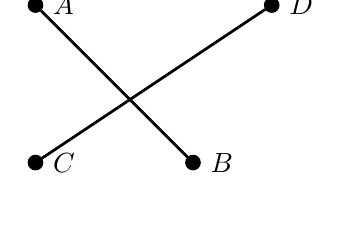
\begin{tikzpicture}
\tkzInit[xmax=4,ymin=1,ymax=4,xmin=0,ymin=0]
\tkzAxeXY
\node[outer sep=0pt,circle, fill,inner 
sep=2pt,label={right:$A$}] (A) at (0,4) {};
\node[outer sep=0pt,circle, fill,inner sep=2pt, 
label={right:$B$}] (B) at (2,2) {};
\node[outer sep=0pt,circle, fill,inner 
sep=2pt,label={right:$C$}] (C) at (0,2) {};
\node[outer sep=0pt,circle, fill,inner sep=2pt, 
label={right:$D$}] (D) at (3,4) {};

\draw[line width=.1em] (A)--(B);
\draw[line width=.1em] (C)--(D);
\end{tikzpicture}

\noindent I. $\overline{CD}$ átfogja-e $\overline{AB}$-t? \\
I/a) {\scshape Forgásirány}$(A,B,C)=\det\Bigg(\begin{bmatrix}
2-0 & 0-0 \\
2-4 & 2-4 \\
\end{bmatrix}\Bigg)=\det\Bigg(\begin{bmatrix}
2  & 0 \\
-2 & -2 \\
\end{bmatrix}\Bigg) = -4 < 0$ \\$\Rightarrow \overrightarrow{AB}$ szakaszhoz 
képest a $C$ csúcs jobbra fordulva érhető el  \\
I/b) {\scshape Forgásirány}$(A,B,D)=\det\Bigg(\begin{bmatrix}
2-0 & 3-0 \\
2-4 & 4-4 \\
\end{bmatrix}\Bigg)=\det\Bigg(\begin{bmatrix}
2  & 3 \\
-2 & 0 \\
\end{bmatrix}\Bigg) = 6 > 0$ \\$\Rightarrow \overrightarrow{AB}$ szakaszhoz 
képest a $D$ csúcs balra fordulva érhető el  \\

\noindent II. $\overline{AB}$ átfogja-e $\overline{CD}$-t? \\
II/c) {\scshape Forgásirány}$(C,D,A)=\det\Bigg(\begin{bmatrix}
3-0 & 0-0 \\
4-2 & 4-2 \\
\end{bmatrix}\Bigg)=\det\Bigg(\begin{bmatrix}
3  & 0 \\
2  & 2 \\
\end{bmatrix}\Bigg) = 6 > 0$ \\$\Rightarrow \overrightarrow{CD}$ szakaszhoz 
képest a $A$ csúcs balra fordulva érhető el  \\
II/d) {\scshape Forgásirány}$(C,D,B)=\det\Bigg(\begin{bmatrix}
3-0 & 2-0 \\
4-2 & 2-2 \\
\end{bmatrix}\Bigg)=\det\Bigg(\begin{bmatrix}
3  & 2 \\
2  & 0 \\
\end{bmatrix}\Bigg) = -4 < 0$ \\$\Rightarrow \overrightarrow{CD}$ szakaszhoz 
képest a $B$ csúcs jobbra fordulva érhető el  \\

I. és II. alapján kijelenthető, hogy az $\overline{AB}$ és $\overline{CD}$ 
szakaszok metszik egymást

\noindent 2. Döntsük el az $A=[0,4], B=[2,2]$, valamint a $C=[1,0], D=[3,3]$ 
végpontokkal adott szakaszokról, hogy metszik-e egymást?

\noindent I. $\overline{AB}$ átfogja-e $\overline{CD}$-t? \\
I/a) {\scshape Forgásirány}$(C,D,A)=\det\Bigg(\begin{bmatrix}
3-1 & 0-1 \\
3-0 & 4-0 \\
\end{bmatrix}\Bigg)=\det\Bigg(\begin{bmatrix}
2  & -1 \\
3  & 4 \\
\end{bmatrix}\Bigg) = 8+3 > 0$ \\$\Rightarrow \overrightarrow{CD}$ szakaszhoz 
képest a $A$ csúcs balra fordulva érhető el  \\
I/b) {\scshape Forgásirány}$(C,D,B)=\det\Bigg(\begin{bmatrix}
3-1 & 2-1 \\
3-0 & 2-0 \\
\end{bmatrix}\Bigg)=\det\Bigg(\begin{bmatrix}
2  & 1 \\
3  & 2 \\
\end{bmatrix}\Bigg) = 6-3 > 0$ \\$\Rightarrow \overrightarrow{CD}$ szakaszhoz 
képest a $B$ csúcs balra fordulva érhető el  \\
$\Rightarrow \overline{AB}$ nem fogja át a $\overline{CD}$-re illeszkedő 
egyenest, így $\overline{AB}$ nem is metszheti $\overline{CD}$-t.

%\textbf{Metsző szakaszpár keresése $O(n \log(n))$-es algoritmussal} ($n$ az 
%összehasonlítandó szakaszok száma).

\noindent 3. Hatékony algoritmussal határozzuk meg, hogy az alábbi szakaszok 
között található-e egymást metsző szakaszpár!

\noindent $\overline{AB}=[(1,5),(4,4)]$ \hfill $\overline{CD}=[(2,5),(5,6)]$ 
\hfill
$\overline{EF}=[(4,3),(8,7)]$ \hfill $\overline{GH}=[(4,7),(7,5)]$ \hfill 
$\overline{IJ}=[(5,3),(7,3)]$

\textbf{Két szakasz összehasonlítása adott $x$ koordináta mentén}\\
$s_1$ szakasz fölötte van $s_2$-nek $x$-nél ($s_1 \succ_x s_2$), ha az $s_1$ 
szakasz $y$-koordinátája nagyobb az $s_2$ szakasz $y$-koordinátájánál az adott 
$x$ koordináta mentén.
Pl. $\overline{GH} \succ_4 \overline{EF}$.

\begin{figure}[h]
\begin{tikzpicture}[scale=.8]
   \tkzInit[xmax=9,ymax=8,xmin=0,ymin=0]
%   \tkzGrid
   \tkzAxeXY
   \node[outer sep=0pt,circle, fill,inner sep=1.5pt,label={[fill=white]left:$A$}] (A) at (1,5) {};
   \node[outer sep=0pt,circle, fill,inner sep=1.5pt, label={[fill=white]right:$B$}] (B) at (4,4) {};
   \node[outer sep=0pt,circle, fill,inner sep=1.5pt,label={[fill=white]left:$C$}] (C) at (2,5) {};
   \node[outer sep=0pt,circle, fill,inner sep=1.5pt, label={[fill=white]right:$D$}] (D) at (5,6) {};
   \node[outer sep=0pt,circle, fill,inner sep=1.5pt,label={[fill=white]left:$E$}] (E) at (4,3) {};
   \node[outer sep=0pt,circle, fill,inner sep=1.5pt, label={[fill=white]right:$F$}] (F) at (8,7) {};
   \node[outer sep=0pt,circle, fill,inner sep=1.5pt,label={[fill=white]left:$G$}] (G) at (4,7) {};
   \node[outer sep=0pt,circle, fill,inner sep=1.5pt, label={[fill=white]right:$H$}] (H) at (7,5) {};
   \node[outer sep=0pt,circle, fill,inner sep=1.5pt,label={[fill=white]left:$I$}] (I) at (5,3) {};
   \node[outer sep=0pt,circle, fill,inner sep=1.5pt, label={[fill=white]right:$J$}] (J) at (7,3) {};
   
   \draw (A)--(B);
   \draw (C)--(D);
   \draw (E)--(F);
   \draw (G)--(H);
   \draw (I)--(J);
   \draw[loosely dotted] (1,0)--(1,8) node[above]{$s_1$};
   \draw[loosely dotted] (2,0)--(2,8) node[above]{$s_2$};
   \draw[loosely dotted] (4,0)--(4,8) node[above]{$s_3$};
   \draw[loosely dotted] (5,0)--(5,8) node[above]{$s_4$};
  \end{tikzpicture}
\end{figure}

Rendezzük a szakaszok végpontjait $x$-koordinátájuk szerint. A holtversenyeket a szakaszok kezdőpontjainak végpontjainak elé sorolásával döntsük el. Az esetleges további holtversenyeket a kisebb $y$-koordinátájú pontok nagyobbak elé sorolásával oldjuk föl. \\
Eredmény: $A,C,E,G,B,I,D,J,H,F$

A szakaszokat tartalmazó kiegyensúlyozott (itt most AVL\footnote{Hf.:piros-fekete fával is végignézni}) keresőfa állapotai a seprőegyenes ($s_i$) haladása szerint.

\begin{enumerate}
\item $s_1$ mentén
 \begin{enumerate}
 \item \texttt{Be(AB)}
 
 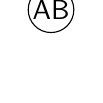
\begin{tikzpicture}[level/.style={sibling distance = 4cm/#1,level distance = 1.3cm}]
 \node[treenode] {AB};
 \end{tikzpicture}
 
 Metszi-e $\overline{AB}$ a fabeli megelőzőjét vagy rákövetkezőjét?
 \end{enumerate}
\item $s_2$ mentén
 \begin{enumerate}
 \item \texttt{Be(CD)}
 
 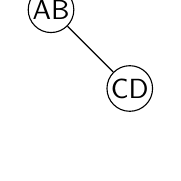
\begin{tikzpicture}
 \node[treenode] {AB} child[missing]{} child{node[treenode] {CD}};
 \end{tikzpicture}
 
  Metszi-e $\overline{CD}$ a fabeli megelőzőjét vagy rákövetkezőjét?
 \end{enumerate}
\item $s_3$ mentén
 \begin{enumerate}
 \item \texttt{Be(EF)}

 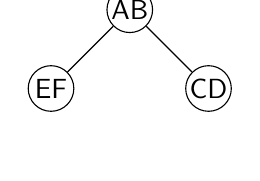
\begin{tikzpicture}
 \node[treenode] {AB} child{node [treenode]{EF}} child{node[treenode] {CD}};
 \end{tikzpicture}

  Metszi-e $\overline{EF}$ a fabeli megelőzőjét vagy rákövetkezőjét?
 \item \texttt{Be(GH)}
 
 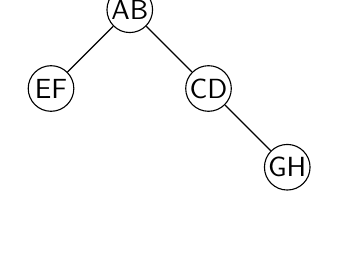
\begin{tikzpicture}
 \node[treenode] {AB} child{node[treenode] {EF}} child{node[treenode] {CD} child[missing]{} child{node[treenode] {GH}}};
 \end{tikzpicture}
 
  Metszi-e $\overline{GH}$ a fabeli megelőzőjét vagy rákövetkezőjét?
 
 \item \texttt{Ki(AB)}
 
  Metszi-e egymást $\overline{AB}$ fabeli megelőzője és rákövetkezője?
 
  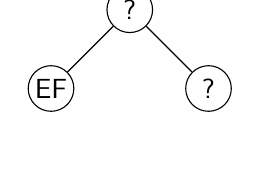
\begin{tikzpicture}
  \node[treenode] {?} child{node [treenode]{EF}} child{node[treenode] {?}};
  \end{tikzpicture}
 
 \end{enumerate}

\item $s_4$ mentén
 \begin{enumerate}
 \item \texttt{Be(IJ)}
 
 Metszi-e $\overline{IJ}$ a fabeli megelőzőjét vagy rákövetkezőjét?
 \end{enumerate}
 
  \begin{enumerate}
  \item \texttt{Ki(CD)}
  
  Metszi-e egymást $\overline{CD}$ fabeli megelőzője és rákövetkezője?
  
  \end{enumerate}
\end{enumerate}

\noindent 4. Határozzuk meg a (1,2), (1,4), (3,3), (4,6), (5,0), (5,3), (5,5), 
(7,5) pontok konvex burkát Graham-féle pásztázással, illetve Jarvis 
meneteléssel!

\paragraph{Graham-féle pásztázás}\mbox{}\\

\noindent I. lépés: csúcsok polárszög szerinti rendezése: A,E,F,C,H,G,D,B. \\
II. lépés: a konvex burok csúcsait nyilvántartó verem fenntartása.
\begin{enumerate}
\item S\textsubscript{0}=[A,E,F] (ekkor még nem kell forgásirányt számoljunk)
\item {\scshape{ForgásIrány(E,F,C)}} S\textsubscript{1}=[A,E,F,C]
\item {\scshape{ForgásIrány(F,C,H)}}, {\scshape{ForgásIrány(E,F,H)}}, 
{\scshape{ForgásIrány(A,E,H)}} S\textsubscript{2}=[A,E,H]
\item {\scshape{ForgásIrány(E,H,G)}} S\textsubscript{3}=[A,E,H,G]
\item {\scshape{ForgásIrány(H,G,D)}}, {\scshape{ForgásIrány(E,H,D)}} 
S\textsubscript{4}=[A,E,H,D]
\item {\scshape{ForgásIrány(H,D,B)}} S\textsubscript{5}=[A,E,H,D,B]
\end{enumerate}

\paragraph{Jarvis menetelés}\mbox{}\\

\noindent I. lépés: legyen $P$ a legbaloldalibb x-koordinátájú pont (a 
pontok $O(n\log{n})$-es rendezésére nincs szükség) \\
II. lépés: amíg vissza nem érünk az elsőnek kiválasztott pontba

válasszuk ki azt a $Q$ pontot, amelyre {\scshape{Forgásirány(P,R,Q)}}>0 minden 
R-re

Adjuk hozzá $Q$-t a konvex burokhoz

P=Q

\begin{table}[b]
\begin{tabular}{ccccc}
1. iteráció & 2. iteráció & 3. iteráció & 4. iteráció & 5. iteráció \\ \hline
FI(A,A,B)=0  & FI(B,A,C)=4 & FI(D,A,E)=22 & FI(H,A,A)=0 & 
\textbf{FI(E,A,F)=-12} \\
FI(A,B,B)=0  & FI(B,B,C)=0 & FI(D,B,E)=20 & FI(H,B,A)=12 & FI(E, B, A)=8 \\
FI(A,C,B)=4  & FI(B,C,C)=0 & FI(D,C,E)=9 & FI(H,C,A)=0 & FI(E, C, A)=8 \\
FI(A,D,B)=6  & \textbf{FI(B,D,C)=-7} & FI(D,D,E)=0 & FI(H,D,A)=15 & FI(E, D, 
A)=22 \\
FI(A,E,B)=8  & FI(B,E,D)=20 & FI(D,E,E)=0 & \textbf{FI(H,E,A)=-24} & FI(E, E, 
A)=0 \\
FI(A,F,B)=8  & FI(B,F,D)=11 & \textbf{FI(D,F,E)=-3} & FI(H,F,E)=6 & FI(E, F, 
A)=12 \\
FI(A,G,B)=8  & FI(B,G,D)=5 & \textbf{FI(D,G,F)=-2} & FI(H,G,E)=10 & FI(E, G, 
A)=20 \\
FI(A,H,B)=12 & FI(B,H,D)=9 & \textbf{FI(D,H,G)=-2} & FI(H,H,E)=0 & FI(E, H, 
A)=24 \\ 
\hline
$B\in CH$ & $D \in CH$ & $H \in CH$ & $E \in CH$ & $A \in CH$ \\
\end{tabular}
\caption{Jarvis menetelése során kiszámított forgásirányok}
\end{table}

\begin{tikzpicture}
\tkzInit[xmax=7,ymin=0,ymax=6,xmin=0,ymin=0]
\tkzAxeXY
   \node[outer sep=0pt,circle, fill,inner 
   sep=1.5pt,label={[fill=white]left:$A$}] (A) at (1,2) {};
\node[outer sep=0pt,circle, fill,inner sep=1.5pt, 
label={[fill=white]right:$B$}] (B) at (1,4) {};
\node[outer sep=0pt,circle, fill,inner sep=1.5pt,label={[fill=white]left:$C$}] 
(C) at (3,3) {};
\node[outer sep=0pt,circle, fill,inner sep=1.5pt, 
label={[fill=white]right:$D$}] (D) at (4,6) {};
\node[outer sep=0pt,circle, fill,inner sep=1.5pt,label={[fill=white]north 
east:$E$}] 
(E) at (5,0) {};
\node[outer sep=0pt,circle, fill,inner sep=1.5pt, 
label={[fill=white]right:$F$}] (F) at (5,3) {};
\node[outer sep=0pt,circle, fill,inner sep=1.5pt,label={[fill=white]left:$G$}] 
(G) at (5,5) {};
\node[outer sep=0pt,circle, fill,inner sep=1.5pt, 
label={[fill=white]right:$H$}] (H) at (7,5) {};

   \draw (A)--(E);
   \draw (E)--(H);
   \draw (H)--(D);
   \draw (D)--(B);
   \draw (B)--(A);
\end{tikzpicture}

\noindent 5. Döntsük el az előző feladat ponthalmazához tartozó zárt nemmetsző 
poligonjához képest az $I=(6,4)$ pont belül vagy kívül helyezkedik-e el!

A zárt nem metsző poligon a csúcsok polárszög szerinti rendezésének 
sorrendjében való összekötésével megkaphatjuk.
Válasszunk egy garantáltan poligonon kívüli $K$ pontot, és vizsgáljuk 
$\overline{IK}$-nak a poligon oldalaival való metszéspontjainak az $m$ számát.

\begin{tikzpicture}
\tkzInit[xmax=7,ymin=0,ymax=6,xmin=0,ymin=0]
\tkzAxeXY
\node[outer sep=0pt,circle, fill,inner 
sep=1.5pt,label={[fill=white]left:$A$}] (A) at (1,2) {};
\node[outer sep=0pt,circle, fill,inner sep=1.5pt, 
label={[fill=white]right:$B$}] (B) at (1,4) {};
\node[outer sep=0pt,circle, fill,inner sep=1.5pt,label={[fill=white]left:$C$}] 
(C) at (3,3) {};
\node[outer sep=0pt,circle, fill,inner sep=1.5pt, 
label={[fill=white]right:$D$}] (D) at (4,6) {};
\node[outer sep=0pt,circle, fill,inner sep=1.5pt,label={[fill=white]north 
	east:$E$}] 
(E) at (5,0) {};
\node[outer sep=0pt,circle, fill,inner sep=1.5pt, 
label={[fill=white]right:$F$}] (F) at (5,3) {};
\node[outer sep=0pt,circle, fill,inner sep=1.5pt,label={[fill=white]left:$G$}] 
(G) at (5,5) {};
\node[outer sep=0pt,circle, fill,inner sep=1.5pt, 
label={[fill=white]right:$H$}] (H) at (7,5) {};
\node[outer sep=0pt,circle, fill,inner sep=1.5pt, 
label={[fill=white]right:$I$}] (I) at (6,4) {};
\node (K) at (0,0) {};

\draw (A)--(E);
\draw (E)--(F);
\draw (F)--(C);
\draw (C)--(H);
\draw (H)--(G);
\draw (G)--(D);
\draw (D)--(B);
\draw (B)--(A);
\draw[color=red] (I)--(K);
\end{tikzpicture}

\end{document}